\documentclass[11pt,a4paper,hidelinks]{article}

\setlength{\headheight}{26pt}

% Packages
\usepackage[left=25mm, right=25mm, top=35mm, bottom=25mm]{geometry} % defines whitespaces on the edges
\usepackage[bottom, hang]{footmisc}
\usepackage{hyperref}             % for \nameref and cite
\usepackage{footnotebackref}      % used for getting back from the footnote to the main text
\usepackage{enumitem}
\usepackage{graphicx}
\usepackage{fancyhdr}
\usepackage{lastpage}
\usepackage[export]{adjustbox}
\usepackage{float}
\usepackage[ngerman]{babel}
\usepackage[ngerman]{datetime}
\usepackage{apacite}
\usepackage[utf8]{inputenc}
\usepackage{listings}
\usepackage{xcolor}
\usepackage{pdfpages}
\usepackage{url}
\usepackage{outlines}
\usepackage{tocloft}
\usepackage[utf8]{inputenc}
\usepackage{amsmath}
\usepackage{mathtools}
\usepackage[acronym]{glossaries}
\usepackage{titlesec}             % for \titleformat
\usepackage{textcomp}             % for \degree sign
\usepackage{gensymb}              % for \degree sign
\usepackage{csvsimple}            % for using csv-files for tables
\usepackage{lscape}               % for landscape mode
\usepackage{parskip}              % inserts space after paragraph automatically
\usepackage{svg}                  % used to include svg with the help of inkscape which converts svg to pdf
\usepackage{wasysym}              % for \diameter symbol
\usepackage{xfrac}                % for \sfrac

\frenchspacing  % Use same space size between words and between sentences

% change section titles' font size
\titleformat*{\section}{\huge\bfseries}
\titleformat*{\subsection}{\LARGE\bfseries}
\titleformat*{\subsubsection}{\Large\bfseries}
\titleformat{\paragraph}[hang]{\large\bfseries}{\theparagraph}{1em}{}
\titleformat{\subparagraph}[hang]{\normalsize\bfseries}{\thesubparagraph}{1em}{}

\definecolor{codegreen}{rgb}{0,0.6,0}
\definecolor{codegray}{rgb}{0.5,0.5,0.5}
\definecolor{codepurple}{rgb}{0.58,0,0.82}
\definecolor{codeorange}{rgb}{1,0.5,0.15}
\definecolor{backcolour}{rgb}{0.9,0.9,0.9}

\lstdefinestyle{mystyle}{
    backgroundcolor=\color{backcolour},
    commentstyle=\color{codegreen},
    keywordstyle=\color{magenta},
    numberstyle=\tiny\color{codegray},
    stringstyle=\color{codepurple},
    basicstyle=\ttfamily\footnotesize,
    breakatwhitespace=false,
    breaklines=true,
    captionpos=b,
    keepspaces=true,
    numbers=left,
    numbersep=5pt,
    showspaces=false,
    showstringspaces=false,
    showtabs=false,
    tabsize=4
}
\lstset{style=mystyle}

\lstset{
    literate={~} {$\sim$}{1}
}

\lstset{%
    breaklines=true,
    breakatwhitespace=true,
}

\DeclarePairedDelimiter\abs{\lvert}{\rvert} % make scalable absolute stripes
\DeclarePairedDelimiter\parenth{(}{)} % make scalable parentheses

\let\phi\varphi{} % change style of \phi sign

\setlength{\parindent}{0mm} % disable paragraph indent

\newdateformat{mydate}{\THEDAY{. }\monthnamengerman[\THEMONTH] \THEYEAR}

\renewcommand{\listfigurename}{}
\renewcommand\contentsname{Inhaltsverzeichnis}
\renewcommand\lstlistingname{Code}

\makeglossaries{}

% Header/Footer Setting
\setlength\footnotemargin{15pt}
\pagestyle{fancy}
\fancyhf{}
\renewcommand{\footrulewidth}{0.4pt} % footer line
\rhead{\textbf{\vUniversity}\\\vModule}
\lhead{\textbf{\vTitle}\\
    Projektarbeit}
\lfoot{\vAuthorFirstName{} \vAuthorLastName}
\cfoot{\mydate\today}
\rfoot{S.~\thepage~/~\pageref{LastPage}}

% Redefine the plain page style, otherwise there is no header and footer for chapter pages
\fancypagestyle{plain}{%
    \fancyhf{}
    \renewcommand{\footrulewidth}{0.4pt} % footer line
    \rhead{\textbf{\vUniversity}\\\vModule}
    \lhead{\textbf{\vTitle}\\
        Projektarbeit}
    \lfoot{\vAuthorFirstName{} \vAuthorLastName}
    \cfoot{\mydate\today}
    \rfoot{S.~\thepage~/~\pageref{LastPage}}
}

\bibliographystyle{apacite}

% Settings for the equation list
\newcommand{\listequationsname}{}
\newlistof{myequations}{equ}{\listequationsname}
\renewcommand{\cftmyequationsaftersnum}{\hfill}
\renewcommand{\cftmyequationspresnum}{\hfill}
\setlength{\cftmyequationsnumwidth}{3.5em}
\newcommand{\myequations}[1]{%
\addcontentsline{equ}{myequations}{\protect\numberline{\theequation}#1}\par}

\newcommand{\mytable}[4]
{
    \centering
    \begin{tabular}{#1}\hline%
        #2 \\ \hline
        \csvreader[
            separator=semicolon,
            head to column names,
            late after line=\\,
        ]{#4}{}{#3}
        \hline
    \end{tabular}
}


% Variables
\newcommand{\vTitle}{DIY Optische ToF Distanzmessung}
\newcommand{\vModule}{CAS Sensorik und Sensor Signal Conditioning}
\newcommand{\vAuthorFirstName}{Matthias Schär,}
\newcommand{\vAuthorLastName}{Timon Burkard}
\newcommand{\vUniversity}{OST -- Ostschweizer Fachhochschule}
\newcommand{\vDegree}{CAS Sensorik und Sensor Signal Conditioning}
\newcommand{\vSemester}{HS24}
\newcommand{\vProfessor}{Prof. Guido Keel}
\newcommand{\vCity}{Rapperswil}
\newcommand{\vAbstract}{Die vorliegende Projektarbeit befasst sich mit der Entwicklung eines\dots}

% Acronyms
\newacronym{pcb}{PCB}{Printed Circuit Board}

\begin{document}

\title{\vspace{-40pt}\begin{huge}\textbf{\vTitle}\end{huge}\\
\ \\ \vModule}
\author{\\\\\textbf{\vAuthorFirstName{} \vAuthorLastName}\\
    \vUniversity{}\\
    \\\\}

\date{\mydate\today}
\maketitle\thispagestyle{empty}  % removes footer from first page

\vspace{35pt}

\begin{figure}[H]
    \centering
    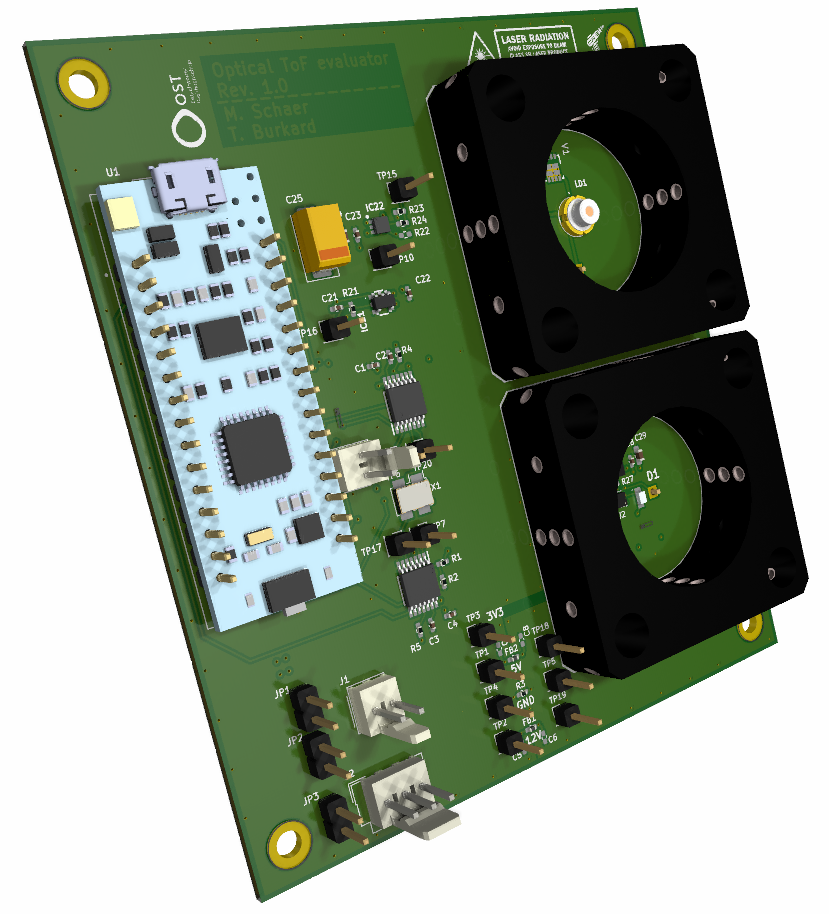
\includegraphics[width=0.6\textwidth]{graphics/cover_picture.png}
\end{figure}

\vspace{30pt}

\begin{figure}[H]
    \centering
    \begin{minipage}[b]{0.3\textwidth}
        \includesvg[width=\textwidth]{graphics/OST_Logo.svg}\label{fig:OST_Logo}
    \end{minipage}
\end{figure}

\pagebreak

\thispagestyle{empty}

\textbf{}
\vspace{5mm}

\begin{flushleft}
    \textbf{\large{\vModule{} an der \vUniversity{}}}
\end{flushleft}

\begin{flushleft}
    \begin{small}
        \begin{tabular}{@{}lll}
            \\
            \textbf{Titel}                 & & \textbf{\vTitle}\\
            \\
            \textbf{Diplomandin/Diplomand} & & \textbf{\vAuthorFirstName{} \vAuthorLastName}\\
            \\
            \textbf{Studiengang}           & & \textbf{\vDegree}\\
            \\
            \textbf{Semester}              & & \textbf{\vSemester}\\
            \\
            \textbf{Dozentin/Dozent}       & & \textbf{\vProfessor}\\
        \end{tabular}
    \end{small}
\end{flushleft}

\vspace{10mm}

% abstracts
\begin{flushleft}
    \begin{small}
        \textbf{Abstract} \\
        \vAbstract{}
        \vspace{15mm}
    \end{small}
\end{flushleft}

% copyright
\begin{flushleft}
    \begin{small}
        Ort, Datum\hspace{30mm}\vCity, \date{\mydate\today} \\
        \textbf{\textcopyright\hspace{1mm}\vAuthorFirstName{} \vAuthorLastName, \vUniversity{}}
    \end{small}
\end{flushleft}

\mbox{}
\vfill

\noindent\makebox[\linewidth]{\rule{\textwidth}{1pt}}
% copyright notice
\begin{flushleft}
    \begin{small}
        Alle Rechte vorbehalten. Die Arbeit oder Teile davon dürfen ohne schriftliche Genehmigung der Rechteinhaber weder in irgendeiner Form reproduziert noch elektronisch gespeichert, verarbeitet, vervielfältigt oder verbreitet werden.\\~\\
        Sofern die Arbeit auf der Website der Ostschweizer Fachhochschule online veröffentlicht wird, können abweichende Nutzungsbedingungen unter Creative-Commons-Lizenzen gelten. Massgebend ist in diesem Fall die auf der Website angezeigte Creative-Commons-Lizenz.
    \end{small}
\end{flushleft}

\pagebreak

\section*{Inhaltsverzeichnis}
\vspace{-25pt}
\renewcommand*\contentsname{}
\tableofcontents

\pagebreak

\section*{Abkürzungsverzeichnis}
\vspace{-25pt}
\printglossary[type=\acronymtype,title={}]

\pagebreak

\section*{Abbildungsverzeichnis}
\vspace{-25pt}
\renewcommand{\listfigurename}{}
\listoffigures

\pagebreak

\section*{Formelverzeichnis}
\vspace{-25pt}
\listofmyequations{}

\pagebreak

\section*{Tabellenverzeichnis}
\vspace{-25pt}
\renewcommand{\listtablename}{}
\listoftables

\pagebreak

\section*{Codeverzeichnis}
\vspace{-33pt}
\renewcommand{\lstlistlistingname}{}
\lstlistoflistings{}

\pagebreak


%%%%%%%%%%%%%%%%%%%%%% CONTENT START %%%%%%%%%%%%%%%%%%%%%%

\section{Ein paar erste Beispiele}\label{sec:beispiel_kapitel}

Lorem ipsum dolor sit amet, consectetur adipiscing elit, sed do eiusmod tempor incididunt ut labore et dolore magna aliqua. Ut enim ad minim veniam, quis nostrud exercitation ullamco laboris nisi ut aliquip ex ea commodo consequat. Duis aute irure dolor in reprehenderit in voluptate velit esse cillum dolore eu fugiat nulla pariatur. Excepteur sint occaecat cupidatat non proident, sunt in culpa qui officia deserunt mollit anim id est laborum.\ \cite{lipsum2022lorem}

\subsection{Abkürzungen}\label{sec:abkuerzungen}

Wir verwenden den Begriff \acrfull{pcb} für eine Leiterplatte. Als Abkürzung verwenden wir \acrshort{pcb}. Wenn man will kann man es aber auch als \acrlong{pcb} ausschreiben.

\subsection{Kapitelverweis}\label{sec:kapitelverweis}

Es kann auf Kapitel verwiesen werden: Siehe Kapitel~\ref{sec:aufzaehlung}.

\subsubsection{Aufzählung}\label{sec:aufzaehlung}

Nachfolgend wird eine einfache Aufzählung gezeigt:

\begin{outline}
    \1 Erstes Element
    \1 Zweites Element
        \2 Unterelement
\end{outline}

\subsubsection{Fussbote}\label{sec:fussnote}

Es können an beliebigen Stellen Fussnoten\footnote{Eine Fussnote ist eine Anmerkung, welche zuunterst auf der Seite aufgeführt wird.} eingefügt werden.

\paragraph{Das ist ein Paragraph}

Nach der subsubsection kommt der paragraph. Dieser ist nicht mehr nummeriert.

\subparagraph{Das ist ein Subparagraph}

Für spezielle Fälle kann auch ein subparagraph verwendet werden.

\pagebreak

\section{Bilder}\label{sec:bilder}

In diesem Kapitel geht es um verschiedene Arten von Bildern. In Abbildung~\ref{fig:example1} ist ein einzelnes Bild dargestellt.

\begin{figure}[H]
    \centering
    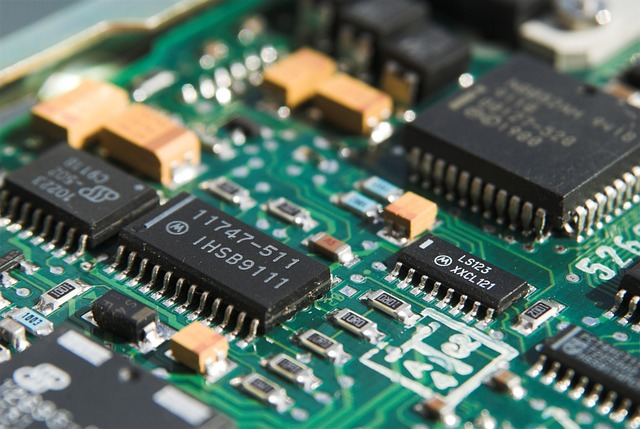
\includegraphics[width=0.5\textwidth]{graphics/example1.jpg}
    \caption[Erstes Beispielbild]{Erstes Beispielbild \cite{pixabay2022pcb}}\label{fig:example1}
\end{figure}

\subsection{Bilder Nebeneinander}\label{sec_literaturreview}

Es können auch Bilder nebeneinander platziert werden, wie in Abbildung~\ref{fig:example2}~und~\ref{fig:example3} dargestellt.

\begin{figure}[H]
    \begin{minipage}[b]{0.48\textwidth}
        \centering
        
\includegraphics[width=\textwidth]{graphics/example2.jpg}
        \caption[Zweites Beispielbild]{Zweites Beispielbild}\label{fig:example2}
    \end{minipage}
    \hfill
    \begin{minipage}[b]{0.48\textwidth}
        \centering
        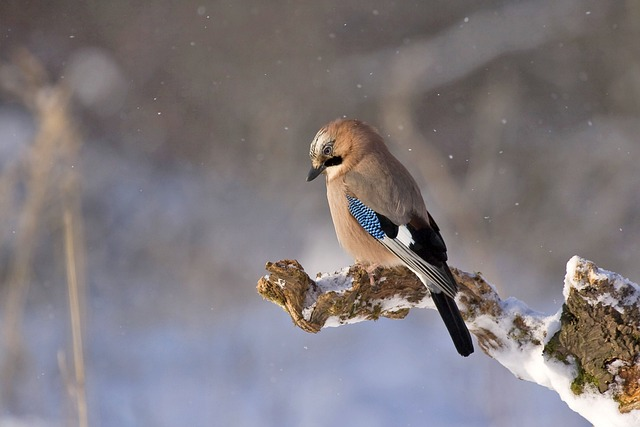
\includegraphics[width=\textwidth]{graphics/example3.jpg}
        \caption[Drittes Beispielbild]{Drittes Beispielbild}\label{fig:example3}
    \end{minipage}
\end{figure}

\subsection{Vektorgrafiken}\label{sec:vektorgrafiken}

Es gibt drei Möglichkeiten, um Vektorgrafiken zu inkludieren.

\subsubsection{SVG Files}\label{sec:svg_files}

Es können SVG Files verwendet werden, wie in Abbildung~\ref{fig:svg_example} gezeigt.

\begin{figure}[H]
    \centering
    \includesvg[width=0.5\textwidth]{graphics/OST_Logo.svg}
    \caption[SVG Beispielbild]{SVG Beispielbild}\label{fig:svg_example}
\end{figure}

\subsubsection{EPS Files}\label{sec:eps_files}

Es können EPS Files verwendet werden, wie in Abbildung~\ref{fig:eps_example} gezeigt.

\begin{figure}[H]
    \centering
    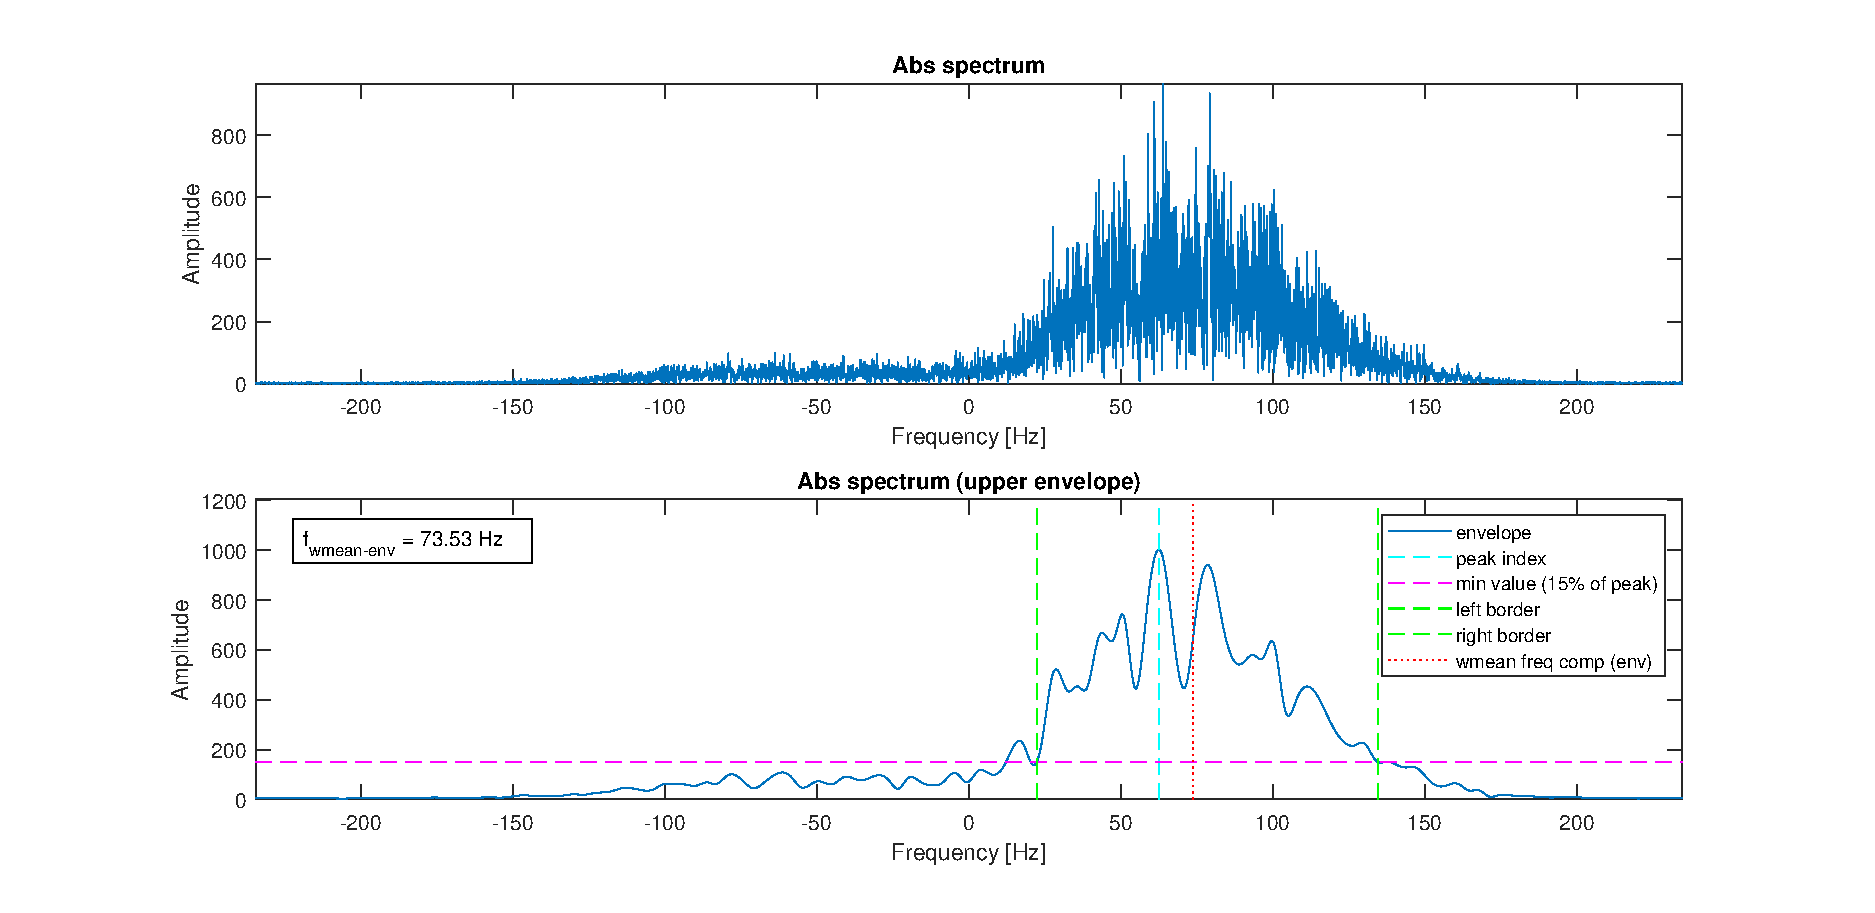
\includegraphics[width=\textwidth]{graphics/eps_example.eps}
    \caption[EPS Beispielbild]{EPS Beispielbild}\label{fig:eps_example}
\end{figure}

\subsubsection{draw.io Files}\label{sec:drawio_files}

Alternativ können auch draw.io Files verwendet werden, wie in Abbildung~\ref{fig:pdf_example} gezeigt. Dies müssen im diagrams/ Verzeichnis sein und werden automatisch in ein PDF konvertiert.

\begin{figure}[H]
    \centering
    \includegraphics[width=\textwidth]{diagrams/drawio_example.pdf}
    \caption[draw.io Beispielbild]{draw.io Beispielbild}\label{fig:pdf_example}
\end{figure}

\section{Formeln}\label{sec:formel}

In Formel~\ref{eq:dopplereffekt_allgemein} \cite{wikipedia2021doppler_effect} ist der Dopplereffekt gezeigt.

\begin{equation}\label{eq:dopplereffekt_allgemein}
    f = \frac{c \pm v_r}{c \pm v_s} \cdot f_0
\end{equation}
\myequations{Formel allgemeiner Dopplereffekt}

Die Berechnung der DFT eines Signales $x[n]$ ist in Formel~\ref{eq:dft} gegeben.

\begin{equation}\label{eq:dft}
    X[k] = \sum^{N-1}_{n=0} x[n] \cdot e^{-j2 \pi n \frac{k}{N}},\qquad k = 0, 1, 2, \dotsb , N-1
\end{equation}
\myequations{Formel zur Berechnung der dft}

$X[k]$ ist das berechnete Frequenzspektrum, welches durch $k$ indexiert wird. $N$ ist die Anzahl Sample des Signals und somit auch die Anzahl Frequenzkomponenten im Spektrum.

\section{Tabelle}\label{sec:tabelle}

In Tabelle~\ref{tab:example} ist eine Tabelle via CSV File gezeigt. Alternativ könnten Tabellen auch direkt im TEX File definiert werden.

\begin{table}[H]
    \mytable
        {|l|c|c|}
        {\textbf{Nr.} & \textbf{Frequenzkomponente [Hz]} & \textbf{Fliessgeschwindigkeit [m/s]}}
        {\nr & \dominantfrequency & \determinedflowspeed}
        {tables/example.csv}
    \caption[Beispieltabelle]{\label{tab:example}Beispieltabelle}
\end{table}

\section{Code}\label{sec:code}

In Code~\ref{code:example} ist ein Beispiel-Code in Matlab gezeigt.

\lstinputlisting[language=matlab, label={code:example}, caption={Matlab-Beispeil}]{sourcecode/example.m}

\section{Anhang}\label{sec:anhang}

Es können auch ganze PDF-Seiten eingefügt werden. Siehe dazu die nachfolgenden zwei Seiten.


\includepdf[pages=1, pagecommand={\subsection{Aufgabenstellung}\label{sec:aufgabenstellung}}, width=\textwidth, frame=true, offset=0 -1cm]{attachments/example.pdf}

\includepdf[pages=2-, pagecommand={}, width=\textwidth, frame=true]{attachments/example.pdf}

%%%%%%%%%%%%%%%%%%%%%% CONTENT END %%%%%%%%%%%%%%%%%%%%%%

\pagebreak

\section*{Quellenverzeichnis}
\begin{flushleft}
\begingroup
\vspace{-25pt}
\renewcommand\refname{}
\renewcommand{\addcontentsline}[3]{} % Do not add bibliography to table of contents, as there is a separate subsection "Quellenverzeichnis"
\bibliography{references}
\endgroup
\end{flushleft}


\end{document}
